\documentclass[11pt, letterpaper]{cmu}

\usepackage[all]{hypcap}
\usepackage[comma,numbers,sort,compress]{natbib}
\usepackage{hyperref}[citecolor=magenta]

\hypersetup{
    colorlinks = true,
    citecolor = {magenta},
}

\usepackage{microtype}
\usepackage{graphicx}
\usepackage{subfigure}
\usepackage{booktabs}
\usepackage{float}

\usepackage{amsmath}
\usepackage{amssymb}
\usepackage{mathtools}
\usepackage{amsthm}
\usepackage{mathrsfs}
\usepackage{nicefrac}
\usepackage{dsfont}
\usepackage{enumitem}
% \usepackage{minted}
\usepackage{float}

\setlength\parindent{0pt}
% \setminted[python]{frame=lines, breaklines, framesep=2mm, fontsize=\footnotesize, numbersep=5pt}

\usepackage{xspace}
\usepackage[capitalize,noabbrev]{cleveref}
\bibliographystyle{plainnat}
\usepackage{subcaption}
\usepackage{wrapfig}
\usepackage{lipsum}
\usepackage{listings}

\usepackage{amsmath}
\usepackage{amssymb}
\usepackage{mathtools}
\usepackage{amsthm}
\usepackage{bbm}
\usepackage{fleqn, tabularx}
\usepackage{multirow}
\usepackage[export]{adjustbox}
\usepackage{colortbl}

\usepackage{algpseudocode}
\usepackage{setspace}

\usepackage{color}
\definecolor{deepblue}{rgb}{0,0,0.5}
\definecolor{deepred}{rgb}{0.6,0,0}
\definecolor{deepgreen}{rgb}{0,0.5,0}
\definecolor{boost_correct_to_correct}{HTML}{66C2A5}
\definecolor{default_correct_to_correct}{HTML}{fc8d62}
\definecolor{dup_correct_to_correct}{HTML}{8da0cb}
\definecolor{new_correct_to_correct}{HTML}{e78ac3}

\newcommand\pythonstyle{\lstset{
basicstyle=\ttfamily\footnotesize,
language=Python,
morekeywords={self, clip, exp, mse_loss, uniform_sample, concatenate, logsumexp},              
keywordstyle=\color{deepblue},
emph={MyClass,__init__},          
emphstyle=\color{deepred},   
stringstyle=\color{deepgreen},
frame=single,                       
showstringspaces=false
}}


\lstnewenvironment{python}[1][]
{
\pythonstyle
\lstset{#1}
}
{}


\newcommand\pythonexternal[2][]{{
\pythonstyle
\lstinputlisting[#1]{#2}}}

\newcommand\pythoninline[1]{{\pythonstyle\lstinline!#1!}}


%% editing comment
\newcommand{\cmt}[1]{{\footnotesize\textcolor{red}{#1}}}
\newcommand{\cmto}[1]{{\footnotesize\textcolor{orange}{#1}}}
\newcommand{\note}[1]{\cmt{Note: #1}}
% \newcommand{\todo}[1]{\cmt{TO-DO: #1}}
\newcommand{\question}[1]{\cmto{Question: #1}}
\newcommand{\ak}[1]{{\textcolor{red}{#1}}}
\newcommand{\aviral}[1]{{\textcolor{red}{#1}}}
\newcommand{\edits}[1]{\textcolor{blue}{#1}}
\newcommand{\editsred}[1]{\textcolor{red}{#1}}
\newcommand{\editsp}[1]{\textcolor{purple}{#1}}
\newcommand{\editsv}[1]{\textcolor{magenta}{#1}}

% \newcommand{\edits}[1]{\textcolor{black}{#1}}
% \newcommand{\editsred}[1]{\textcolor{black}{#1}}
% \newcommand{\editsp}[1]{\textcolor{black}{#1}}
% \newcommand{\editsv}[1]{\textcolor{black}{#1}}


%% abbreviations
\newcommand{\x}{\mathbf{x}}
\newcommand{\z}{\mathbf{z}}
\newcommand{\y}{\mathbf{y}}
\newcommand{\w}{\mathbf{w}}
\newcommand{\data}{\mathcal{D}}
\newcommand{\E}{\mathbb{E}}

\newcommand{\etal}{{et~al.}\ }
\newcommand{\eg}{\emph{e.g.},\ }
\newcommand{\ie}{\emph{i.e.},\ }
\newcommand{\nth}{\text{th}}
\newcommand{\pr}{^\prime}
\newcommand{\tr}{^\mathrm{T}}
\newcommand{\inv}{^{-1}}
\newcommand{\pinv}{^{\dagger}}
\newcommand{\real}{\mathbb{R}}
\newcommand{\gauss}{\mathcal{N}}
% \newcommand{\norm}[1]{\left|#1\right|}
% \newcommand{\trace}{\text{tr}}

%% specifics for the paper
\newcommand{\reward}{r}
\newcommand{\policy}{\pi}
\newcommand{\mdp}{\mathcal{M}}
\newcommand{\states}{\mathcal{S}}
\newcommand{\actions}{\mathcal{A}}
\newcommand{\observations}{\mathcal{O}}
\newcommand{\transitions}{T}
\newcommand{\initstate}{d_0}
\newcommand{\freq}{d}
\newcommand{\obsfunc}{E}
\newcommand{\initial}{\mathcal{I}}
\newcommand{\horizon}{H}
\newcommand{\rewardevent}{R}
\newcommand{\probr}{p_\rewardevent}
\newcommand{\metareward}{\bar{\reward}}
\newcommand{\discount}{\gamma}
\newcommand{\behavior}{{\pi_\beta}}
\newcommand{\bellman}{\mathcal{B}}
\newcommand{\qparams}{\phi}
\newcommand{\qparamset}{\Phi}
\newcommand{\qset}{\mathcal{Q}}
\newcommand{\batch}{B}
\newcommand{\qfeat}{\mathbf{f}}
\newcommand{\Qfeat}{\mathbf{F}}
\newcommand{\hatbehavior}{\hat{\pi}_\beta}

\newcommand{\traj}{\tau}

\newcommand{\pihi}{\pi^{\text{hi}}}
\newcommand{\pilo}{\pi^{\text{lo}}}
\newcommand{\ah}{\mathbf{w}}

% \newcommand{\proj}{\Pi}

\newcommand{\loss}{\mathcal{L}}
\newcommand{\eye}{\mathbf{I}}

\newcommand{\model}{\hat{p}}

\newcommand{\pimix}{\pi_{\text{mix}}}

\newcommand{\pib}{\bar{\pi}}
\newcommand{\epspi}{\epsilon_{\pi}}
\newcommand{\epsmodel}{\epsilon_{m}}

\newcommand{\return}{\mathcal{R}}

%% math
\newcommand{\cY}{\mathcal{Y}}
\newcommand{\cX}{\mathcal{X}}
\newcommand{\en}{\mathcal{E}}
\newcommand{\bu}{\mathbf{u}}
\newcommand{\bv}{\mathbf{v}}
% \newcommand{\bb}{\mathbf{b}}
\newcommand{\bd}{\mathbf{d}}
\newcommand{\be}{\mathbf{e}}
\newcommand{\by}{\mathbf{y}}
\newcommand{\bx}{\mathbf{x}}
\newcommand{\bz}{\mathbf{z}}
\newcommand{\bw}{\mathbf{w}}
\newcommand{\boldm}{\mathbf{m}}
\newcommand{\bo}{\mathbf{o}}
% \newcommand{\bs}{\mathbf{s}}
% \newcommand{\ba}{\mathbf{a}}
\newcommand{\bs}{\mathbf{s}}
\newcommand{\ba}{\mathbf{a}}
\newcommand{\bM}{\mathbf{M}}
\newcommand{\ot}{\bo_t}
% \newcommand{\st}{\bs_t}
\newcommand{\at}{\ba_t}
\newcommand{\op}{\mathcal{O}}
\newcommand{\opt}{\op_t}
\newcommand{\kl}{D_\text{KL}}
\newcommand{\tv}{D_\text{TV}}
\newcommand{\ent}{\mathcal{H}}
\newcommand{\bG}{\mathbf{G}}
\newcommand{\byk}{\mathbf{y_k}}
\newcommand{\bI}{\mathbf{I}}
\newcommand{\bg}{\mathbf{g}}
\newcommand{\bV}{\mathbf{V}}
\newcommand{\bD}{\mathbf{D}}
\newcommand{\bR}{\mathbf{R}}
\newcommand{\bQ}{\mathbf{Q}}
\newcommand{\bA}{\mathbf{A}}
\newcommand{\bN}{\mathbf{N}}
\newcommand{\bS}{\mathbf{S}}
\newcommand{\bW}{\mathbf{W}}
\newcommand{\bU}{\mathbf{U}}
\newcommand{\bO}{\mathbf{O}}
\newcommand{\leftnorm}{\left\vert \left\vert}
\newcommand{\rightnorm}{\right\vert \right\vert}

\newcommand{\bzhi}{\bz^\text{hi}}
\newcommand{\expected}{\mathbb{E}}
% \newcommand{\srank}{\text{srank}}
% \newcommand{\rank}{\text{rank}}
\newcommand{\deepnet}{\bW_N(k, t) \bW_\phi(k, t)}
\newcommand{\features}{\bW_\phi(k, t)}
\newcommand{\stateactioni}{[\bs_i; \ba_i]}
% \newcommand{\diag}{\text{\textbf{diag}}}
\newcommand{\cosine}{\text{cos}}


\def\thetaP{\theta^{\prime}}
\def\cf{\emph{c.f.}\ }
\def\vs{\emph{vs}.\ }
\def\etc{\emph{etc.}\ }
\def\Eqref#1{Equation~\ref{#1}}
\def\ss#1{\scriptsize #1}

\newenvironment{repeatedthm}[1]{\@begintheorem{#1}{\unskip}}{\@endtheorem}

% \DeclareMathOperator\supp{supp}
\newcommand{\methodname}{Cal-QL}
\newcommand{\aliasingproblemname}{bootstrapping aliasing}
\newcommand{\Aliasingproblemname}{Bootstrapping aliasing}
\newcommand{\AliasingProblemName}{Bootstrapping Aliasing}
\newcommand{\simnorm}{\mathrm{sim}_{\mathrm{n}}^\pi}
\newcommand{\simunnorm}{\mathrm{sim}_{\mathrm{u}}^\pi}

% colors from moderncv that are especially appealing
\definecolor{blanchedalmond}{rgb}{1.0, 0.92, 0.8}
\definecolor{carmine}{rgb}{0.59, 0.0, 0.09}
\definecolor{lightblue}{rgb}{0.22,0.45,0.70}% light blue


\newcommand{\gjt}[1]{\textcolor{red}{[gjt: #1]}}
% \newcommand{\rebuttal}[1]{\textcolor{red}{#1}}
\newcommand{\rebuttal}[1]{#1}
\newcommand{\scenario}[1]{\textcolor{lightblue}{S#1}}
\newcommand{\technique}[1]{\textcolor{carmine}{T#1}}
\newcommand{\application}[1]{\textcolor{carmine}{A#1}}

\def\bellmanop{T^\circ}
\def\qop{Q^\circ}
\def\qpi{Q^\pi}
\def\qs{Q^*}
\def\Qstar{Q^*}
\def\Qt{Q_{\theta}}
\def\Qtp{Q_{\thetaP}}
\def\ld{\ell_{\lambda}}


%%% SZ.1.11: added my math defs below:

\newtheorem{theorem}{Theorem}[section]
\newtheorem{sketchtheorem}{Sketch Theorem}[section]
\newtheorem{lemma}[theorem]{Lemma}
\newtheorem{corollary}[theorem]{Corollary}
\newtheorem{proposition}[theorem]{Proposition}
\newtheorem{definition}[theorem]{Definition}
\newtheorem{conjecture}[theorem]{Conjecture}
\newtheorem{problem}[theorem]{Problem}
\newtheorem{formulation}[theorem]{Formulation}
\newtheorem{claim}[theorem]{Claim}
\newtheorem{remark}[theorem]{Remark}
\newtheorem{example}[theorem]{Example}
\newtheorem{assumption}[theorem]{Assumption}
\newtheorem{exercise}[theorem]{Exercise}


\newcommand{\indep}{\rotatebox[origin=c]{90}{$\models$}}

\renewcommand{\mathbf}{\boldsymbol}

\newcommand{\conv}{\circledast}
\newcommand{\mb}{\mathbf}
\newcommand{\mc}{\mathcal}
\newcommand{\mf}{\mathfrak}
\newcommand{\md}{\mathds}
\newcommand{\bb}{\mathbb}
\newcommand{\msf}{\mathsf}
\newcommand{\mcr}{\mathscr}
\newcommand{\magnitude}[1]{ \left| #1 \right| }
\newcommand{\set}[1]{\left\{ #1 \right\}}
\newcommand{\condset}[2]{ \left\{ #1 \;\middle|\; #2 \right\} }


\newcommand{\reals}{\bb R}
\newcommand{\proj}{\mathrm{proj}}

\newcommand{\eps}{\varepsilon}
\newcommand{\R}{\reals}
\newcommand{\Cp}{\bb C}
\newcommand{\Z}{\bb Z}
\newcommand{\N}{\bb N}
\newcommand{\Sp}{\bb S}
\newcommand{\Ba}{\bb B}
\newcommand{\indicator}[1]{\mathbbm 1\left\{#1\right\}}
\renewcommand{\P}{\mathbb{P}}
\newcommand{\rvline}{\hspace*{-\arraycolsep}\vline\hspace*{-\arraycolsep}}
\makeatletter
\def\Ddots{\mathinner{\mkern1mu\raise\p@
\vbox{\kern7\p@\hbox{.}}\mkern2mu
\raise4\p@\hbox{.}\mkern2mu\raise7\p@\hbox{.}\mkern1mu}}
\makeatother
% to declare new operator
% \DeclareMathOperator{\xxx}{xxx}

%% Other definitions

\newcommand{\event}{\mc E}

\newcommand{\e}{\mathrm{e}}
\newcommand{\im}{\mathrm{i}}
\newcommand{\rconcave}{r_\fgecap}
\newcommand{\Lconcave}{\mc L^\fgecap}
\newcommand{\rconvex}{r_\fgecup}
\newcommand{\Rconvex}{R_\fgecup}
\newcommand{\Lconvex}{\mc L^\fgecup}

\newcommand{\wh}{\widehat}
\newcommand{\wt}{\widetilde}
\newcommand{\ol}{\overline}


\newcommand{\betaconcave}{\beta_\fgecap}
\newcommand{\betagrad}{\beta_{\mathrm{grad}}}

\newcommand{\norm}[2]{\left\| #1 \right\|_{#2}}
\newcommand{\abs}[1]{\left| #1 \right|}
\newcommand{\row}[1]{\text{row}\left( #1 \right)}
\newcommand{\innerprod}[2]{\left\langle #1,  #2 \right\rangle}
\newcommand{\prob}[1]{\bb P\left[ #1 \right]}
\newcommand{\expect}[1]{\bb E\left[ #1 \right]}
\newcommand{\function}[2]{#1 \left(#2\right}
\newcommand{\integral}[4]{\int_{#1}^{#2}\; #3\; #4}
\newcommand{\paren}[1]{\left( #1 \right)}
\newcommand{\brac}[1]{\left[ #1 \right]}
\newcommand{\Brac}[1]{\left\{ #1 \right\}}

% Adding new defs here
\newcommand{\moff}{m_\mr{off}}
\newcommand{\mon}{m_\mr{on}}
\newcommand{\EmpiricalOffline}{\wh{\bb E}_{\mc D^\nu_h}}
\newcommand{\EmpiricalOnline}{\wh{\bb E}_{\mc D^\tau_h}}
\newcommand{\Deltaoff}{\Delta_\mr{off}}
\newcommand{\Deltaon}{\Delta_\mr{on}}
\newcommand{\Vmax}{V_{\max}}
\newcommand{\regret}{\mr{Reg}}
\newcommand{\regreton}{\mr{Sub}_{\mr {on}}}
\newcommand{\regretoff}{\mr{Sub}_{\mr {off}}}
\newcommand{\Doff}{\mc D_\mr{off}}
\newcommand{\Don}{\mc D_\mr{on}}
\newcommand{\piref}{\pi_\mr{ref}}

\newcommand{\nt}[1]{{\color{purple}{\bf [Next: #1]}}}
\newcommand{\here}{{\color{purple}{\bf [Writing here]}}}
% \newcommand{\todo}{{\color{purple}{\bf [TODO]}}}
\newcommand{\sz}[1]{{\color{blue}{\bf [Simon: #1]}}}
% \newcommand{\note}[1]{{\color{red}{\bf [note: #1]}}}
\newcommand{\mr}{\mathrm}
\newcommand{\sym}{\mathrm{Sym}}
\newcommand{\sks}{\mathrm{Skew}}
\newcommand{\inprod}[2]{\langle#1,#2\rangle}
\newcommand{\parans}[1]{\left(#1\right}
\newcommand{\clip}{\msf{clipped}}
\newcommand{\beha}{\msf b}
\numberwithin{equation}{section}

\definecolor{amaranth}{rgb}{0.9, 0.17, 0.31}
\definecolor{antiquebrass}{rgb}{0.8, 0.58, 0.46}
\definecolor{antiquefuchsia}{rgb}{0.57, 0.36, 0.51}
% \definecolor{chromeyellow}{rgb}{1.0, 0.65, 0.0}
% \definecolor{chromeyellow}{rgb}{0.82, 0.41, 0.12}
% \definecolor{chromeyellow}{rgb}{1.0, 0.5, 0.31}
\definecolor{chromeyellow}{rgb}{0.31, 0.47, 0.26}


\def \endprf{\hfill {\vrule height6pt width6pt depth0pt}\medskip}
% \newenvironment{proof}{\noindent {\bf Proof} }{\endprf\par}

% \newcommand{\qed}{{\unskip\nobreak\hfil\penalty50\hskip2em\vadjust{}
%            \nobreak\hfil$\Box$\parfillskip=0pt\finalhyphendemerits=0\par}}

%% table color
\usepackage[dvipsnames]{xcolor}
% \definecolor{maj5}{HTML}{009ADE}
% \definecolor{maj5Imp}{HTML}{0D4A70}
\definecolor{maj5}{HTML}{2b8cbe}
\definecolor{maj5Imp}{HTML}{084081}

\definecolor{seq5wo}{HTML}{d95f0e}
\definecolor{seq5woImp}{HTML}{662506}

\definecolor{seq5w}{HTML}{6a51a3}
\definecolor{seq5wImp}{HTML}{3f007d}

\definecolor{selfwo}{HTML}{d95f0e}
\definecolor{selfwoImp}{HTML}{662506}

\definecolor{selfw}{HTML}{6a51a3}
\definecolor{selfwImp}{HTML}{3f007d}

\definecolor{glorewo}{HTML}{d95f0e}
\definecolor{glorewoImp}{HTML}{662506}

\definecolor{glorew}{HTML}{6a51a3}
\definecolor{glorewImp}{HTML}{3f007d}

% \definecolor{selfw}{HTML}{00718B}
% \definecolor{selfwImp}{HTML}{003147}

% \definecolor{selfwo}{HTML}{E32977}
% \definecolor{selfwoImp}{HTML}{8F003B}

% \definecolor{glorew}{HTML}{00718B}
% \definecolor{glorewImp}{HTML}{003147}

% \definecolor{glorewo}{HTML}{E32977}
% \definecolor{glorewoImp}{HTML}{8F003B}

\definecolor{vstar}{HTML}{d95f0e}
\definecolor{vstarImp}{HTML}{662506}








\makeatletter
\def\mathcolor#1#{\@mathcolor{#1}}
\def\@mathcolor#1#2#3{%
  \protect\leavevmode
  \begingroup
    \color#1{#2}#3%
  \endgroup
}
\makeatother

\usepackage[textsize=tiny]{todonotes}
\usepackage{algorithm}
\usepackage{amssymb}


\usepackage[skins,theorems]{tcolorbox}
\Crefformat{equation}{#2Eq.\;(#1)#3}

\Crefformat{figure}{#2Figure #1#3}
\Crefformat{assumption}{#2Assumption #1#3}
\Crefname{assumption}{Assumption}{Assumptions}

\usepackage{crossreftools}
\pdfstringdefDisableCommands{
    \let\Cref\crtCref
    \let\cref\crtcref
}
\newcommand{\creftitle}[1]{\crtcref{#1}}

\usepackage[suppress]{color-edits}

\newcommand\numberthis{\addtocounter{equation}{1}\tag{\theequation}}

\usepackage{dsfont}
\usepackage{nicefrac}

\newtcolorbox{analysisbox}[1][]{
    enhanced jigsaw,
    colback=white,
    colframe=blue!75!black,
    fonttitle=\bfseries,
    boxsep=5pt,
    left=5pt,
    right=5pt,
    top=5pt,
    bottom=5pt,
    title=#1,
}
\newcommand{\mistake}[1]{\sethlcolor{highlightmistake}\hl{#1}\sethlcolor{yellow}}
\newcommand{\correct}[1]{\sethlcolor{highlightcorrect}\hl{#1}\sethlcolor{yellow}}
\newcommand{\cmark}{\ding{51}}
\newcommand{\xmark}{\ding{55}}

\tcbset{
  aibox/.style={
    width=\linewidth,
    top=8pt,
    bottom=4pt,
    colback=blue!6!white,
    colframe=black,
    colbacktitle=black,
    enhanced,
    center,
    attach boxed title to top left={yshift=-0.1in,xshift=0.15in},
    boxed title style={boxrule=0pt,colframe=white,},
  }
}
\newtcolorbox{AIbox}[2][]{aibox,title=#2,#1}
\definecolor{lightblue}{rgb}{0.22,0.45,0.70}% light blue

\usepackage{pifont}
\usepackage{soul}
\definecolor{highlightmistake}{RGB}{255, 179, 179}
\definecolor{highlightcorrect}{RGB}{179, 255, 179} 
\newcommand{\rr}[1]{\textbf{\color{green}[RR: #1]}}

\title{Safe-f2o: Failure-efficient Offline-to-Online RL Fine-tuning with a Budgeted Expert}

% \reportnumber{} 

\author[1]{Yizhou Wang}
\author[1]{Melody Gao}

\affil[1]{Carnegie Mellon University}

\correspondingauthor{Your email}

\hyphenation{pre-print}

\begin{abstract}
Online RL fine-tuning of an offline-pretrained policy is costly mainly because of online failures,
such as a robot falling over. This is especially frequent if the offline behavior is suboptimal.
We investigate whether adding a budgeted expert who takes over when the policy is unreliable
can reduce the number of online
terminations needed to reach the same return. So far, on MuJoCo Ant (Minari \texttt{medium} data), we have trained an offline TD3+BC
policy and fine-tuned it online with an unlimited budget. Fine-tuning raises the return from about 600 to about 4300,
at a cost of about 270 terminations; this run is both our baseline and our expert. Keeping BC
regularisation online was essential. In a rollout of the offline policy, $Q$ drops about 10 steps
before a fall, which supports $Q$-based gating. Code: \url{https://github.com/Burgundy800020/co_cal}.
\end{abstract}

\begin{document}

\maketitle

\section{Project Overview and Motivation}
Briefly restate your original project goal and motivation. 
What problem are you addressing, and why is it important? 
Has your problem formulation changed since the proposal? If yes, describe why.

\textbf{Goal and motivation.}
Offline-to-online RL fine-tunes an offline-pretrained policy through online interaction, but in real
deployments every online failure (e. g. a crashed robot) is costly. We aim to match the return
of standard fine-tuning while incurring far fewer online terminations, by spending a limited expert
budget only when the learner is unreliable.

\textbf{Change in formulation.}
Yes, our formulation has changed. The proposal focused on conformally calibrating an offline policy 
so that we could detect when it is unreliable. We realized that this detection signal is more useful 
in a more actionable setting: online RL fine-tuning, where the costly events are online 
failures/terminations. We therefore now ask whether a budgeted 
expert, who intervenes when the learner is unreliable, can let us fine-tune an offline policy 
online to the same performance at much lower failure cost. This turns a purely diagnostic question into 
one with a clear payoff.



\section{Progress and Technical Work So Far [13 points]}
Describe your technical progress to date.
\begin{itemize}
    \item What models, algorithms, or systems have you implemented?
    \item What preliminary experiments have you run? Include early results, plots, or tables.
    \item Highlight key insights, unexpected results, or implementation challenges.
\end{itemize}

So far we have finished the first two stages of our pipeline on Ant: offline pretraining and
unlimited-budget offline-to-online (O2O) fine-tuning. The O2O run is both our main baseline and the
source of the expert for stage three.

\textbf{Stage 1: offline TD3+BC.}
We implemented TD3+BC~\cite{fujimoto2021minimalist}. Its actor loss is
$-\lambda\, Q(s,\pi(s)) + w_{\text{BC}}\,\|\pi(s)-a\|^2$ with $\lambda = \alpha / \overline{|Q|}$, and it
normalises states using dataset statistics. The weight $w_{\text{BC}}$ lets us move smoothly from
TD3+BC ($w_{\text{BC}}=1$) to plain TD3 ($w_{\text{BC}}=0$) during fine-tuning. On Ant we trained for
20k gradient steps ($\alpha=4$, learning rate $3\cdot10^{-4}$, $256\times256$ MLPs) on the \texttt{medium}
dataset (\cref{fig:offline_ant}). The policy reaches an evaluation return of
$1041 \pm 1194$ over 20 episodes. The very large spread is the important part: some episodes
reach $\sim$5000, while many end almost immediately because the ant falls over. This makes it
a good starting point for fine-tuning: it is good enough to be worth fine-tuning but still fails often.

\begin{figure}[H]
    \centering
    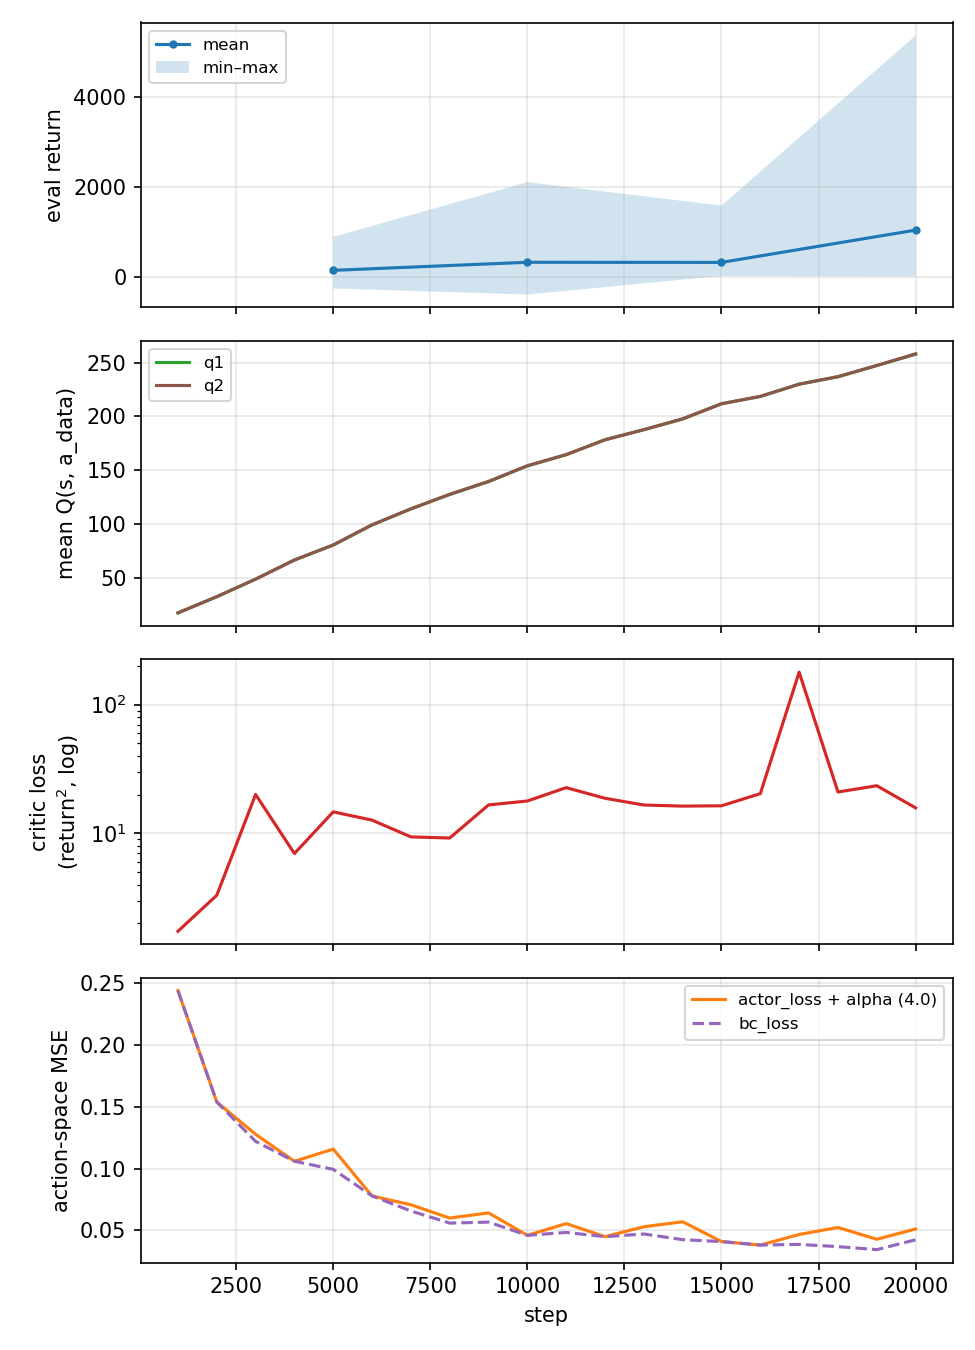
\includegraphics[width=0.45\linewidth]{figures/td3bc_ant_medium_training.png}
    \caption{Offline TD3+BC on \texttt{ant/medium-v0}. From top to bottom: evaluation return (mean and min--max over 20 episodes),
    mean $Q$ on dataset actions, critic loss, and actor/BC loss.}
    \label{fig:offline_ant}
\end{figure}

\textbf{Stage 2: offline-to-online fine-tuning (unlimited budget).}
We built an environment-agnostic online loop that tracks the cumulative number of online terminations,
our cost axis. Only true failures count, not time-limit truncations. The loop takes a pluggable
reset function, which we will later use to start episodes from expert handover states. We start
from the offline \texttt{medium} checkpoint with fresh Adam optimisers (learning rate $10^{-4}$, $\alpha=1$).
The offline data stays in the replay buffer, and each batch is half offline and half online, as in
RLPD~\cite{ball2023efficient}. Before updating the actor, we run 5k critic-only steps so that the critic
can adapt to online data. The BC weight is annealed from 0.5 to 0.3 over 200k environment steps,
with exploration noise 0.1 and an update-to-data ratio of 1.

\Cref{fig:o2o_ant} shows the results over 5 seeds. Fine-tuning raises the evaluation return from
$601 \pm 62$ to $4313 \pm 159$ in 200k steps. This costs $271 \pm 23$ online terminations, out of
about 380 episodes, so roughly 70\% of training episodes end with the robot falling. 
Terminations pile up fastest at the start (about 60
in the first 25k steps), when the policy is weakest. This is exactly where a budgeted expert should
help most. The fine-tuned policy ($\sim$4300 return) will serve as the expert in stage three.

\begin{figure}[H]
    \centering
    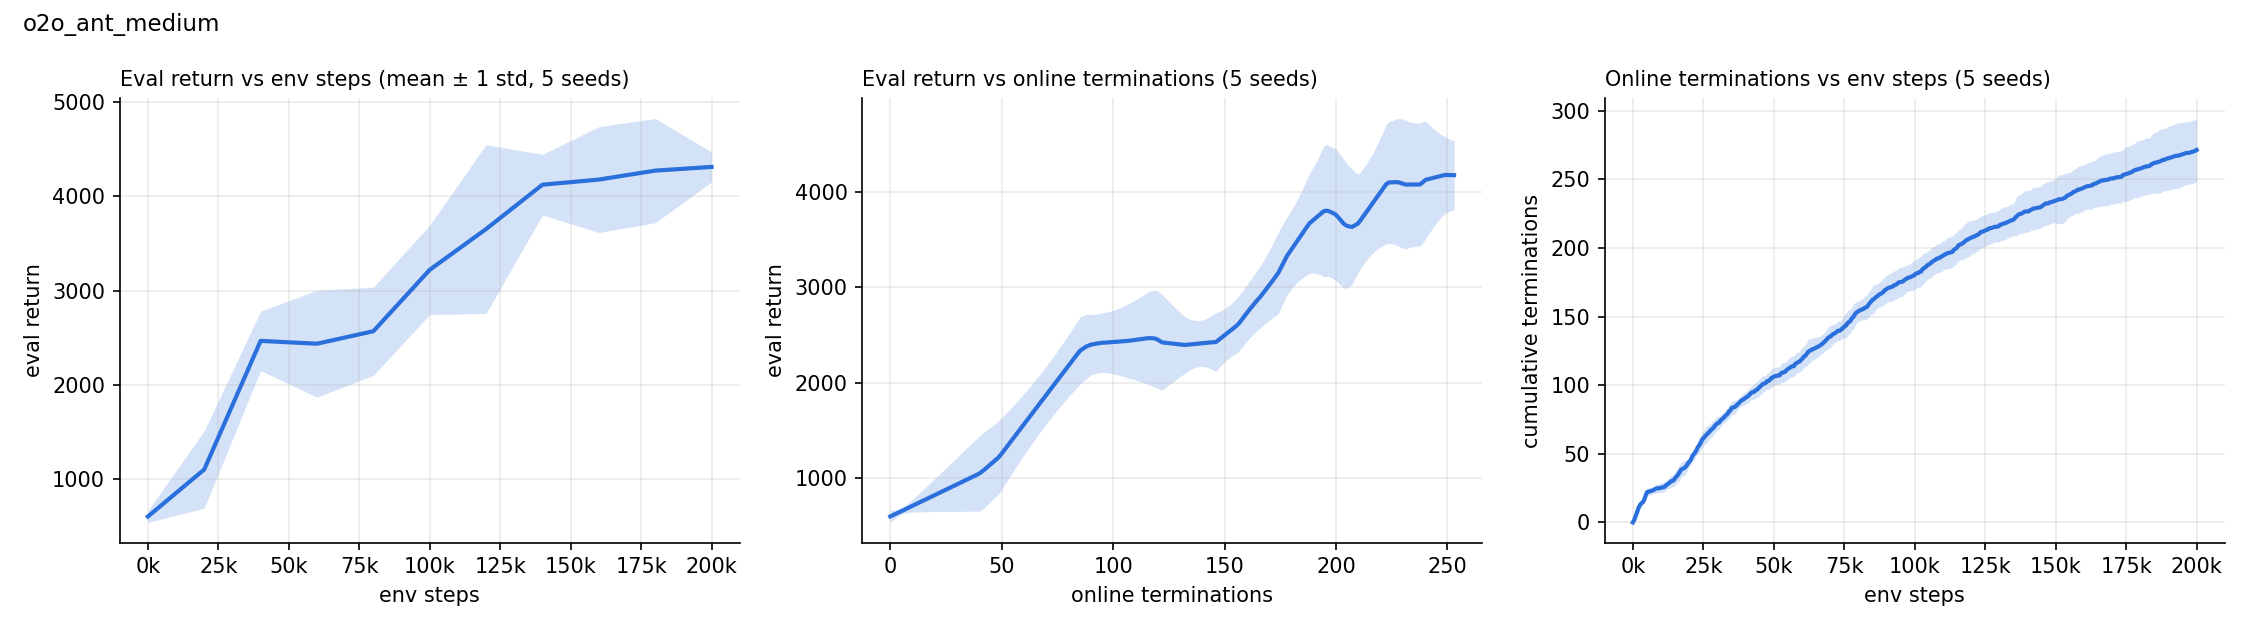
\includegraphics[width=\linewidth]{figures/o2o_ant_medium_seeds.png}
    \caption{Unlimited-budget O2O fine-tuning from offline TD3+BC on \texttt{ant/medium-v0} (5 seeds,
    mean $\pm$ 1 std). Left: evaluation return vs.\ environment steps. Middle: evaluation return vs.\
    cumulative online terminations, our key metric. Right: cumulative terminations vs.\ environment steps.}
    \label{fig:o2o_ant}
\end{figure}

\textbf{Can $Q$ pre-detect failures?}
To check whether $Q$ is a usable unreliability signal, we recorded the offline policy rolling out on
Ant with $Q(s,\pi(s))$ overlaid on each frame (video in \cref{app:video}).
The ant falls and the episode terminates after about 250 steps, and $Q$ visibly drops about 10 steps
\emph{before} the termination. This is only a single qualitative example, but it suggests the critic can
flag unreliable states early enough for an expert to take over before the failure happens, which is
the premise of our method.

\begin{AIbox}{Takeaways box}
% \footnotesize
With suboptimal offline data, the offline policy may sit near a local optimum, and offline-to-online
fine-tuning faces a choice between two strategies:
\begin{enumerate}[leftmargin=*, itemsep=0pt]
    \item \textbf{Keep BC regularisation online.} Learning is stable, but performance is bounded
    near the local optimum that the offline policy and data define.
    \item \textbf{Drop BC regularisation.} The policy can in principle escape that optimum, but it suffers
    an early performance dip and risks degenerating into online RL from scratch, which wastes the
    offline pretraining and causes many failures.
\end{enumerate}
On Ant-medium we tried both with our specific offline checkpoint, and only strategy 1 worked. We therefore
keep a BC weight (annealed from 0.5 to 0.3), which reaches a return of $\sim$4300.

\smallskip
In a rollout of the offline policy, $Q$ drops about 10 steps before the ant falls. This suggests
$Q$ can flag an unreliable policy early enough for a budgeted expert to step in.
\end{AIbox}


\section{Datasets, Environments, and Resources [2 points]}
\begin{itemize}
    \item Describe datasets or simulation environments used.
    \item Mention any preprocessing, environment setup, or modifications.
    \item Report approximate compute usage (e.g., GPU hours or cluster nodes).
\end{itemize}

\textbf{Datasets and environments.}
We use the Minari MuJoCo datasets (\texttt{mujoco/\{ant, walker2d\}/\{simple, medium\}-v0})
for offline pretraining. The matching Gymnasium MuJoCo environments (recovered from the datasets so that versions
and settings match) are used for online fine-tuning. This is because Ant and Walker2d have true
failure terminations (the robot falls or becomes unhealthy).

\textbf{Preprocessing and setup.}
We normalise states using the mean and standard deviation of the offline dataset and apply the same
statistics online. Only true terminations stop bootstrapping and count as online failures; time-limit
truncations do not. During fine-tuning, the offline data stays in the replay buffer, and each batch draws
half its samples from offline data and half from online data.

\textbf{Compute.}
Everything runs on CPU on a laptop. Each offline TD3+BC run takes a few
minutes. A 200k-step online fine-tuning run takes about 10--15 minutes (around 300 env steps/s).

\section{Updated Plan and Next Steps [5 points]}
Summarize your plan for the remainder of the semester.
\begin{itemize}
    \item What remains to be done (e.g., final experiments, analysis, writing)?
    \item What are your next milestones and expected timeline?
    \item Identify potential risks or blockers and mitigation strategies.
\end{itemize}

\textbf{Remaining work.}
Stages 1 and 2 are done on Ant-medium. What remains is stage 3, our method: online TD3 fine-tuning
in which a $Q$-gated expert (the fine-tuned policy) takes over for a few steps under a fixed
intervention budget, plus online BC on the expert steps. We will compare it with the unlimited-budget
O2O baseline and with DAgger, plotting return vs.\ online terminations.

\textbf{Timeline.}
\begin{itemize}[itemsep=0pt]
    \item \textbf{Week 1:} Implement the expert-intervention loop (gating, handover, and BC on expert
    steps) and the $Q$ threshold calibration. Run first single-seed tests on Ant-medium.
    \item \textbf{Week 2:} Run the full 5-seed comparison against O2O and DAgger, plus a sweep over intervention
    budgets. Make the video and poster for the presentation at the \textbf{end of week 2}.
    \item \textbf{Week 3:} Run ablations of the gating signal and BC on expert steps, run a second environment
    (Walker2d) if time allows, and write the \textbf{final report} at the \textbf{end of week 3}.
\end{itemize}

\textbf{Risks and mitigation.}
(1) The scale of $Q$ shifts early in fine-tuning, so a fixed threshold may trigger interventions poorly.
We will try relative or normalised $Q$ signals and recalibrate on recent online data.
(2) $Q$ may give no warning before many failures, beyond the single rollout in \cref{app:video}.
We will first measure how often and how early $Q$ drops before terminations, and we will fall back on
other uncertainty signals (e.g., critic disagreement) if it is unreliable. (3) Time is short, so Ant-medium takes priority, and other environments are optional.

\section{Team Contributions}
List major responsibilities of each member (implementation, experiments, writing, etc.), 
and describe any changes in team organization or workload balance.

\begin{itemize}
    \item \textbf{Yizhou Wang:} Experimental design. Reformulated the project around failure-efficient offline-to-online
    fine-tuning and the return-vs.-terminations metric.
    Ideated the $Q$-based intervention signal.
    \item \textbf{Melody Gao:} Code implementation and experiments. Run 
    experiments across environments, hyperparameters, and seeds.
\end{itemize}

\section{Reflection and Feedback}
Discuss what you have learned so far, what challenges remain, 
and what feedback or support you would like from the course staff (e.g., technical feedback, compute, additional readings).

\textbf{What we learned.}
With suboptimal offline data, offline-to-online fine-tuning involves a real trade-off between keeping BC
regularisation, which is stable but bounded by the offline policy, and dropping it, which risks a collapse
into learning from scratch. On Ant, only the regularised option worked. We also saw early evidence
that $Q$ drops shortly before a failure, which supports using it as the intervention signal.

\textbf{Remaining challenge: a moving $Q$ scale.}
At the start of online fine-tuning, the critic adapts to online data and the overall scale of
$Q$ shifts. As a result, a fixed threshold calibrated offline no longer tells us what counts as a
``low'' $Q$, and the intervention trigger can fire too often, wasting budget, or too rarely, letting
failures through. We are considering relative signals (e.g., a drop in $Q$ along the trajectory, or
$Q$ normalised by a running estimate of its scale) and periodically recalibrating the threshold on recent
online data, as ThriftyDAgger~\cite{hoque2021thriftydagger} does with its risk threshold.

\textbf{Feedback requested.}
We would most value feedback on our research design. Is the offline-to-online setting, with
``return vs.\ number of online terminations'' as the key metric, the best way to evaluate
failure-efficient fine-tuning? Is using a fine-tuned policy as the budgeted expert a reasonable proxy
for a human or safe controller? 






\bibliography{main}

\newpage
\appendix
\onecolumn
\part*{Appendices}

\section{Rollout video with $Q$-values}
\label{app:video}
\url{https://drive.google.com/file/d/1elGXkT-8ZKsVjD1gcoxnqWIkKPHW9N3e/view?usp=sharing}

The video shows one rollout of the offline TD3+BC policy on \texttt{ant/medium-v0}, with
$Q(s,\pi(s))$ overlaid on each frame. The ant falls and the episode terminates after about 250 steps,
and $Q$ drops about 10 steps before the termination.

\end{document}